\documentclass[11pt,a4paper]{article}
\usepackage[utf8]{inputenc}
\usepackage[T1]{fontenc}
\usepackage[english]{babel}
\usepackage{lmodern}
\usepackage{microtype}
\usepackage{geometry}
\usepackage{graphicx}
\usepackage{xcolor}
\usepackage{hyperref}
\usepackage{tikz}
\usepackage{float}
\usepackage{booktabs}
\usetikzlibrary{arrows.meta,positioning}

% Ajustes básicos de estilo
\geometry{margin=2.5cm}
\setlength{\parskip}{0.6em}
\setlength{\parindent}{0pt}
\graphicspath{{./figuras/}}
\hypersetup{
  colorlinks=true,
  linkcolor=blue!60!black,
  urlcolor=blue!60!black,
  citecolor=blue!60!black
}

\title{Implementation of custom HMM for Basque and Catalan\\\large Computational Syntax}
\author{Josu Bayer, Ane Paniagua, Ander Pe\~na, Be\~nat Alkain}
\date{\today}

\begin{document}
\maketitle
\tableofcontents
\bigskip

\section{Introduction}
Part-of-speech tagging assigns a syntactic role to each token (e.g., DET, NOUN, VERB) so that well-formed transitions such as ADJ\,$\rightarrow$\,NOUN or NOUN\,$\rightarrow$\,VERB emerge while unlikely ones are penalized. In this project we frame tagging as a generative sequence problem with Hidden Markov Models.

Our goal is to implement and evaluate a custom HMM tagger on two Universal Dependencies corpora (Basque and Catalan) to test robustness across a highly agglutinative language and a more fusional one. We compare against the reference HMM in \texttt{nltk} and backoff n-gram baselines (unigram, bigram, trigram), using token-level accuracy on train/dev/test and per-tag breakdowns over the 17 universal categories. This report follows the grading axes: correct HMM implementation, sound experiments on two datasets, and analysis of results.

\section{Methodology}
We use the Universal Dependencies corpora for Basque and Catalan, each provided as CSV with parallel \textit{text} and \textit{tags} fields. Sentences are tokenized at whitespace and paired word-by-word with their UPOS labels (17-tag inventory). Data are split into train/dev/test partitions; train drives parameter estimation, dev is used for model comparison, and test reports final generalization. Table~\ref{tab:csv-ud} shows sample rows from the Basque training split to illustrate the schema and the morpho-syntactic granularity of the tags.

\begin{table}[H]
  \centering
  \caption{UD CSV structure (Basque train split).}
  \label{tab:csv-ud}
  \small
  \begin{tabular}{p{2cm}p{4cm}p{9cm}}
    \hline
    sentence\_id & text & tags \\
    \hline
    train-s1 & Gero , lortutako masa molde batean jarri . & ADV PUNCT VERB NOUN NOUN NUM VERB PUNCT \\
    train-s2 & Bestalde , `` herri palestinarrari laguntza tekniko eta ekonomikoa ematen jarraitzeko ... baieztatu zuen EBk . & CCONJ PUNCT NOUN ADJ NOUN ADJ CCONJ ADJ VERB VERB CCONJ NOUN ADJ CCONJ ADJ NUM NOUN AUX NOUN ADJ VERB NOUN VERB NOUN PUNCT VERB AUX PROPN PUNCT \\
    \hline
  \end{tabular}
\end{table}

The core model is a Hidden Markov Model that factorizes the joint sequence probability as \(p(x, y) = p(y)\,p(x\mid y)\). Transition probabilities \(p(y_i\mid y_{i-1})\) and emission probabilities \(p(x_i\mid y_i)\) are estimated by maximum likelihood counts over the training set, with explicit initial-state probabilities for sentence starts. The MLE parameter estimation and Viterbi decoding are implemented in \texttt{model/hmm.py} (methods \texttt{train} and \texttt{viterbi}), and the evaluation helpers for accuracy and per-tag accuracy live in \texttt{main.py}.

We train two implementations: (i) the reference \texttt{nltk} HMM tagger; (ii) our own HMM implementation using the same MLE recipe and Viterbi decoding as above. We also build backoff n-gram baselines (default, unigram, bigram, trigram) to quantify the benefit of sequential context over context-free tagging.

Evaluation is token-level accuracy on train/dev/test for both languages, complemented with per-tag accuracy to identify categories with higher error (e.g., infrequent or ambiguous tags). We also inspect POS frequency distributions to anticipate sparsity effects, and run qualitative Viterbi examples to verify that predicted tag transitions align with plausible syntactic sequences.

\begin{figure}[H]
  \centering
  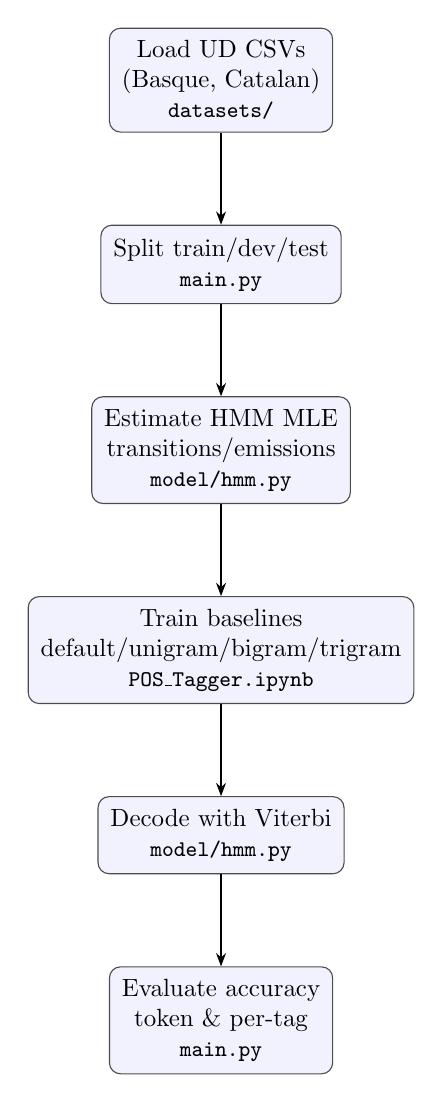
\begin{tikzpicture}[>=Stealth, node distance=1.3cm, every node/.style={rectangle, rounded corners, draw=black!70, fill=blue!5, align=center, inner sep=5pt}, scale=0.9, transform shape]
    \node (load) {Load UD CSVs\\(Basque, Catalan)\\\small \texttt{datasets/}};
    \node (split) [below=of load] {Split train/dev/test\\\small \texttt{main.py}};
    \node (train) [below=of split] {Estimate HMM MLE\\transitions/emissions\\\small \texttt{model/hmm.py}};
    \node (baseline) [below=of train] {Train baselines\\default/unigram/bigram/trigram\\\small \texttt{POS\_Tagger.ipynb}};
    \node (decode) [below=of baseline] {Decode with Viterbi\\\small \texttt{model/hmm.py}};
    \node (eval) [below=of decode] {Evaluate accuracy\\token \& per-tag\\\small \texttt{main.py}};
    \draw[->] (load) -- (split);
    \draw[->] (split) -- (train);
    \draw[->] (train) -- (baseline);
    \draw[->] (baseline) -- (decode);
    \draw[->] (decode) -- (eval);
  \end{tikzpicture}
  \caption{Methodological flow: data ingestion to evaluation with code pointers.}
\end{figure}

\section{Results}
\subsection{Overall accuracy by split and language}
Figure~\ref{fig:acc-eu} and Figure~\ref{fig:acc-ca} compare token accuracy of the reference \texttt{nltk} HMM and our custom HMM on train/dev/test for Basque and Catalan. Numerically, for Basque we obtain 0.9569/0.8258/0.8189 (train/dev/test) with NLTK and 0.9693/0.8622/0.8560 with our HMM; for Catalan 0.9703/0.9453/0.9430 versus 0.9761/0.9477/0.9445. The dev–test gap is larger in Basque (e.g., 0.8622\(\rightarrow\)0.8560) than in Catalan (0.9477\(\rightarrow\)0.9445), reflecting higher sparsity from agglutinative morphology.

\begin{figure}[H]
  \centering
  \includegraphics[width=0.8\linewidth]{hmm_accuracy_eu.png}
  \caption{Basque: accuracy of NLTK HMM vs. custom HMM on train/dev/test.}
  \label{fig:acc-eu}
\end{figure}

\begin{figure}[H]
  \centering
  \includegraphics[width=0.8\linewidth]{hmm_accuracy_ca.png}
  \caption{Catalan: accuracy of NLTK HMM vs. custom HMM on train/dev/test.}
  \label{fig:acc-ca}
\end{figure}

\subsection{Comparison with n-gram baselines}
Backoff taggers encode bounded context (unigram/bigram/trigram), while HMMs model the joint \(p(x, y)\) combining transitions and emissions. On the Basque test set the n-gram taggers reach 0.859 (unigram), 0.866 (bigram) and 0.866 (trigram), slightly above our HMM (0.8560) but ahead of the NLTK HMM (0.8189). For Catalan, n-grams reach 0.921/0.935/0.935, clearly below the NLTK HMM (0.9430) and ours (0.9445). Figure~\ref{fig:ngram} visualizes these differences when combining plausible transitions (e.g., ADJ\(\rightarrow\)NOUN) with emissions.

\begin{figure}[H]
  \centering
  \includegraphics[width=0.8\linewidth]{ngram_vs_hmm.png}
  \caption{Token accuracy: default/unigram/bigram/trigram vs. HMMs (Basque split).}
  \label{fig:ngram}
\end{figure}

\subsection{Per-tag analysis}
Figures~\ref{fig:per-tag-eu} and \ref{fig:per-tag-ca} detail per-tag accuracies for our HMM. Although the bars vary by tag, the quantitative pattern is consistent: closed classes (DET, ADP, AUX, PUNCT) cluster at the top, while open classes (NOUN, VERB, PROPN, ADV) drop. In Basque the drop is sharper due to larger vocabulary and sparser emissions; in Catalan the spread is milder.

\begin{figure}[H]
  \centering
  \includegraphics[width=0.95\linewidth]{pos_accuracy_eu.png}
  \caption{Per-tag accuracy of our HMM on the Basque test set.}
  \label{fig:per-tag-eu}
\end{figure}

\begin{figure}[H]
  \centering
  \includegraphics[width=0.95\linewidth]{pos_accuracy_ca.png}
  \caption{Per-tag accuracy of our HMM on the Catalan test set.}
  \label{fig:per-tag-ca}
\end{figure}

\subsection{Per-tag bars and comparisons}
Grouped bar charts from the classification reports summarize precision/recall/F1 by tag. Figures~\ref{fig:per-tag-bars-nltk-eu}–\ref{fig:per-tag-bars-nltk-ca} (NLTK) and \ref{fig:per-tag-bars-ours-eu}–\ref{fig:per-tag-bars-ours-ca} (ours) show how scores spread across tags; Figures~\ref{fig:per-tag-compare-eu}–\ref{fig:per-tag-compare-ca} compare F1 directly between models. Our HMM lifts most tags over NLTK in both languages, matching the macro-F1 gains reported numerically. Full confusion matrices are provided in Appendix~\ref{app:confusion}.

\begin{figure}[H]
  \centering
  \includegraphics[width=0.7\linewidth]{per_tag_nltk_eu.png}
  \caption{Per-tag precision/recall/F1 (NLTK HMM, Basque). Higher variance across tags.}
  \label{fig:per-tag-bars-nltk-eu}
\end{figure}

\begin{figure}[H]
  \centering
  \includegraphics[width=0.7\linewidth]{per_tag_nltk_ca.png}
  \caption{Per-tag precision/recall/F1 (NLTK HMM, Catalan).}
  \label{fig:per-tag-bars-nltk-ca}
\end{figure}

\begin{figure}[H]
  \centering
  \includegraphics[width=0.7\linewidth]{per_tag_our_eu.png}
  \caption{Per-tag precision/recall/F1 (Our HMM, Basque). Closed classes dominate; open classes drop.}
  \label{fig:per-tag-bars-ours-eu}
\end{figure}

\begin{figure}[H]
  \centering
  \includegraphics[width=0.7\linewidth]{per_tag_our_ca.png}
  \caption{Per-tag precision/recall/F1 (Our HMM, Catalan). More uniform than Basque.}
  \label{fig:per-tag-bars-ours-ca}
\end{figure}

\begin{figure}[H]
  \centering
  \includegraphics[width=0.7\linewidth]{compare_reports_eu.png}
  \caption{Per-tag F1 comparison: Our HMM vs NLTK (Basque). Gains concentrated in frequent tags.}
  \label{fig:per-tag-compare-eu}
\end{figure}

\begin{figure}[H]
  \centering
  \includegraphics[width=0.7\linewidth]{compare_reports_ca.png}
  \caption{Per-tag F1 comparison: Our HMM vs NLTK (Catalan). Broad improvements with small gaps.}
  \label{fig:per-tag-compare-ca}
\end{figure}

\subsection{Qualitative checks}
The joint probability for a Basque test sentence was \(4.29\times 10^{-13}\), consistent with multiplying probabilities over long sequences. Random samples from the HMM show plausible tag alternations (ADJ\(\rightarrow\)NOUN\(\rightarrow\)VERB), reinforcing the generative interpretation.

\subsection{Basque test metrics}
Running \texttt{main.py} on the Basque test set yields 0.85595 accuracy. Table~\ref{tab:eu-metrics} summarizes precision/recall/F1 by tag; macro-F1 is 0.772 (macro recall 0.745) and weighted-F1 0.854, reflecting drops in rare classes (INTJ, SCONJ, X) and stability in frequent/closed ones (PUNCT, PART, CCONJ).

\begin{table}[H]
  \centering
  \caption{Basque test set: precision/recall/F1 by tag.}
  \label{tab:eu-metrics}
  \small
  \begin{tabular}{lccc}
    \toprule
    Tag & Precision & Recall & F1 \\
    \midrule
    ADJ   & 0.914 & 0.626 & 0.743 \\
    ADP   & 0.879 & 0.911 & 0.895 \\
    ADV   & 0.939 & 0.818 & 0.874 \\
    AUX   & 0.773 & 0.900 & 0.832 \\
    CCONJ & 0.956 & 0.986 & 0.971 \\
    DET   & 0.959 & 0.917 & 0.938 \\
    INTJ  & 0.500 & 0.125 & 0.200 \\
    NOUN  & 0.798 & 0.853 & 0.824 \\
    NUM   & 0.996 & 0.781 & 0.876 \\
    PART  & 0.990 & 0.997 & 0.993 \\
    PRON  & 1.000 & 0.827 & 0.906 \\
    PROPN & 0.831 & 0.662 & 0.737 \\
    PUNCT & 0.936 & 1.000 & 0.967 \\
    SCONJ & 0.000 & 0.000 & 0.000 \\
    SYM   & 1.000 & 1.000 & 1.000 \\
    VERB  & 0.812 & 0.823 & 0.817 \\
    X     & 0.769 & 0.435 & 0.556 \\
    \midrule
    \textbf{Macro-F1}     & \multicolumn{3}{c}{0.772 (macro recall 0.745)} \\
    \textbf{Weighted-F1}  & \multicolumn{3}{c}{0.854} \\
    \textbf{Accuracy}     & \multicolumn{3}{c}{0.85595} \\
    \bottomrule
  \end{tabular}
\end{table}

\subsection{Catalan test metrics}
Running \texttt{main.py} on the Catalan test set yields 0.94479 accuracy. Table~\ref{tab:ca-metrics} summarizes precision/recall/F1 by tag; macro-F1 is 0.836 (macro recall 0.827) and weighted-F1 0.944, showing higher overall performance and fewer drops on rare classes compared to Basque.

\begin{table}[H]
  \centering
  \caption{Catalan test set: precision/recall/F1 by tag.}
  \label{tab:ca-metrics}
  \small
  \begin{tabular}{lccc}
    \toprule
    Tag & Precision & Recall & F1 \\
    \midrule
    ADJ   & 0.906 & 0.870 & 0.888 \\
    ADP   & 0.980 & 0.993 & 0.986 \\
    ADV   & 0.927 & 0.949 & 0.938 \\
    AUX   & 0.949 & 0.985 & 0.967 \\
    CCONJ & 0.988 & 0.992 & 0.990 \\
    DET   & 0.951 & 0.990 & 0.970 \\
    INTJ  & 0.000 & 0.000 & 0.000 \\
    NOUN  & 0.928 & 0.953 & 0.940 \\
    NUM   & 0.922 & 0.824 & 0.870 \\
    PART  & 1.000 & 0.190 & 0.320 \\
    PRON  & 0.907 & 0.851 & 0.878 \\
    PROPN & 0.924 & 0.832 & 0.876 \\
    PUNCT & 0.984 & 0.992 & 0.988 \\
    SCONJ & 0.776 & 0.916 & 0.840 \\
    SYM   & 0.990 & 0.981 & 0.986 \\
    VERB  & 0.954 & 0.919 & 0.936 \\
    \midrule
    \textbf{Macro-F1}     & \multicolumn{3}{c}{0.836 (macro recall 0.827)} \\
    \textbf{Weighted-F1}  & \multicolumn{3}{c}{0.944} \\
    \textbf{Accuracy}     & \multicolumn{3}{c}{0.94479} \\
    \bottomrule
  \end{tabular}
\end{table}

\section{Conclusions}
\begin{itemize}
  \item Our HMM edges the \texttt{nltk} HMM in both languages: +3.6 test points in Basque (0.8560 vs. 0.8189) and +0.15 in Catalan (0.9445 vs. 0.9430), with dev gains of 0.8622 vs. 0.8258 (EU) and 0.9477 vs. 0.9453 (CA).
  \item Against backoff n-gram taggers, Basque trigram hits 0.866 (slightly above our HMM 0.8560 and well above \texttt{nltk} 0.8189); in Catalan the HMMs lead over n-grams (0.9445/0.9430 vs. 0.935). Joint modeling of transitions and emissions yields a clear advantage in CA and is on par in EU.
  \item Language effect: Basque shows larger train\(\rightarrow\)dev/test drops (0.9693\(\rightarrow\)0.8622\(\rightarrow\)0.8560) than Catalan (0.9761\(\rightarrow\)0.9477\(\rightarrow\)0.9445), reflecting how agglutinative morphology increases \(p(x\mid y)\) sparsity.
  \item Tag-wise (Basque test): PUNCT 1.000, PART 0.997, and CCONJ 0.986 lead; open classes dip (NOUN 0.853, VERB 0.823, PROPN 0.662) and rare tags drop sharply (INTJ 0.125, X 0.435, SCONJ 0.000). In Catalan, overall scores rise (accuracy 0.94479, macro-F1 0.836): closed classes stay high (ADP 0.986 F1, PUNCT 0.988 F1), and open classes improve (NOUN 0.940 F1, VERB 0.936 F1), with only INTJ and PART showing low recall (0.000 and 0.190).
  \item Confusion matrices align with these patterns: diagonals are cleaner in Catalan than Basque, and our HMM reduces off-diagonal mass compared to \texttt{nltk}, especially for frequent tags.
  \item Per-tag bars and F1 comparisons confirm gains across most tags for our HMM over NLTK in both languages, consistent with higher macro-F1 (EU 0.772 vs. 0.745 macro recall; CA 0.836 vs. 0.827 macro recall).
  \item Sequential probability: the joint probability for a Basque example was \(4.29\times 10^{-13}\), a reasonable scale for long sequences; random samples and Viterbi paths confirm the model favors well-formed tag orders.
\end{itemize}

\appendix
\section{Confusion matrices}
\label{app:confusion}

\begin{figure}[H]
  \centering
  \includegraphics[width=0.7\linewidth]{confusion_hmm_eu.png}
  \caption{Confusion matrix for our HMM (Basque). Strong diagonal; confusions mostly in open classes.}
  \label{fig:conf-hmm-eu}
\end{figure}

\begin{figure}[H]
  \centering
  \includegraphics[width=0.7\linewidth]{confusion_hmm_ca.png}
  \caption{Confusion matrix for our HMM (Catalan). Cleaner diagonal than Basque, reflecting fewer inflectional variants.}
  \label{fig:conf-hmm-ca}
\end{figure}

\begin{figure}[H]
  \centering
  \includegraphics[width=0.7\linewidth]{confusion_nltk_eu.png}
  \caption{Confusion matrix for NLTK HMM (Basque). Off-diagonal mass is higher than our HMM.}
  \label{fig:conf-nltk-eu}
\end{figure}

\begin{figure}[H]
  \centering
  \includegraphics[width=0.7\linewidth]{confusion_nltk_ca.png}
  \caption{Confusion matrix for NLTK HMM (Catalan). Less noise than Basque, but still below our HMM.}
  \label{fig:conf-nltk-ca}
\end{figure}

\end{document}
